%%% Image: Google panorama
\begin{figure}[t]
  \begin{minipage}{0.3\linewidth}
    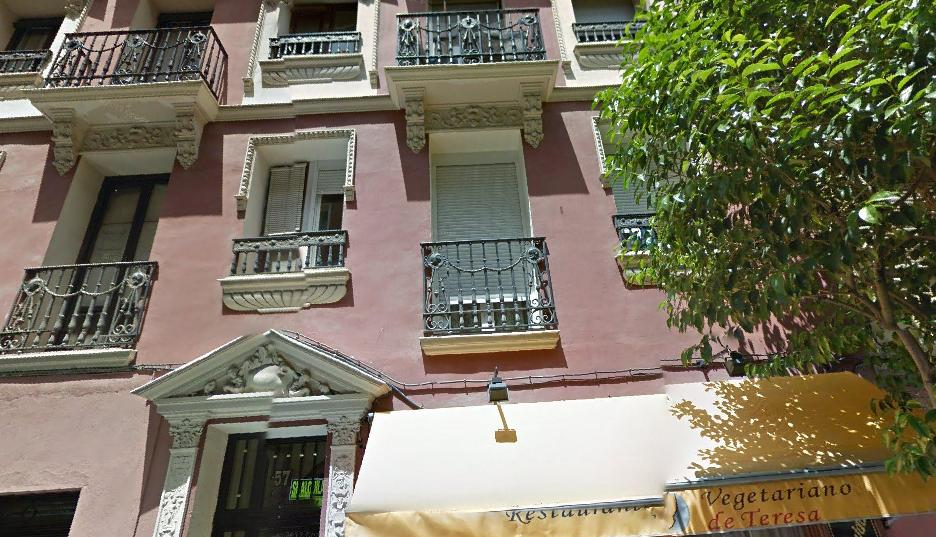
\includegraphics[width=\linewidth]{imgs/cutout_pitch28.jpg} \\ \vspace{-3.5mm} \\
    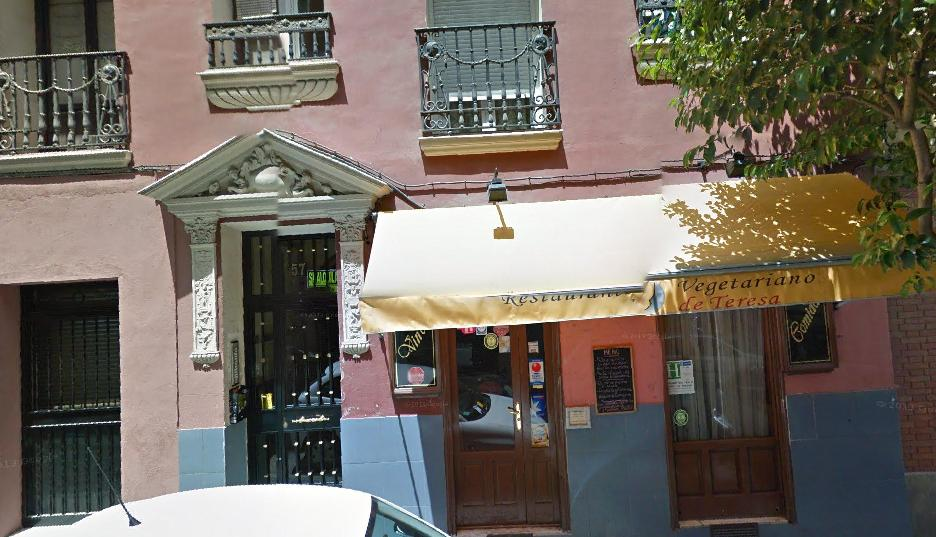
\includegraphics[width=\linewidth]{imgs/cutout_pitch04.jpg}
  \end{minipage}
  %
  \begin{minipage}{0.7\linewidth}
    \begin{overpic}[width=\textwidth]{imgs/panorama.jpg}
      %%% Lines
      \linethickness{0.15mm}
        \put(50,0){\color{blue}\vector(0,1){50}}  %center line
      {\color{red}
        \put(25,0){\color{red}\vector(0,1){50}}   % left line
        \put(75,0){\color{red}\vector(0,1){50}}   % right line
        \multiput(12.5,-6)(0,2){28}                    % FOV left
          {\line(0,1){1}}
        \multiput(37.5,-6)(0,2){28}                    % FOV right
          {\line(0,1){1}} 
        \put(12.5,-4.5){\vector(1,0){25}}
        \put(37.5,-4.5){\vector(-1,0){25}}
      }
      %%% Text
      \put(21,-8){\color{black} \scriptsize FOV $90^\circ$}
      \put(47,-3){\color{black} \scriptsize Google}
      \put(44,-6){\color{black} \scriptsize car direction}
      \put(21,-3){\color{black} \scriptsize left side}
      \put(71,-3){\color{black} \scriptsize right side}
    \end{overpic}
  \end{minipage}
  %
  \vspace{5mm}
  \caption{
  A center of each panorama \emph{(right)} corresponds to the Google car motion. For each side of the panorama we generate two perspective images \emph{(left)} with horizontal field of view $90^\circ$ in two different elevation pitches in order to capture both street view level and building facades.
  }
  \label{fig:pano}
\end{figure}